
\chapter{緒論}
自從網際網路的誕生以來,各式各樣的服務與應用也迅速的蓬勃發展,商品與服務的數位化,已經大大改變了人們的生活習慣。而如何將貨幣數位化一直是個熱門的議題。但面臨如何解決偽造和重複支付一直是個重大挑戰。與網路訊息一樣,數位貨幣只是單純的一串訊息,如何確定使用者擁有該數位貨幣,且交易事件是無法逆轉改變的,是非常重要的問題。在比特幣\cite{Bitcoin}被發明之前,常見的方法是建立一個人們共同信任的第三方機構,例如:中央政府或金融企業等,來協助交易的清算以及交易記錄的保存。同時確保該交易發生後,帳戶餘額是正確的。這類做法雖然頗具效率,但是賦予第三方機構過大權力卻可能導致不好的結果,例如:國家能夠透過加印鈔票,來稀釋鈔票的價值,進而控制金融市場,或是遊戲公司也可能透過發行新的虛擬點數,讓原先的虛擬點數一文不值。

區塊鏈技術則能解決上述過於依賴第三方者的問題,我們稱區塊鏈系統中的每一位參與者為節點,區塊鍊是一種基於分散式系統的節點備份技術,系統中所有的節點共同維護與更新同一份帳本資料,且每一個節點都會各自保留一份小備份,節點間的權力相互平等,沒有第三者來管理秩序。在分散式網路裡,區塊鏈內各節點所看到的帳本內容,是一致且順序相同的。一條完整的區塊鏈,是由連續的區塊所組成。區塊內記錄了一段時間內各個節點所提交的儲存內容(通常為多筆交易)。區塊內還包含該區塊產生的時間戳,該時間戳與前幾個區塊的時間戳不能差距過大,這使得惡意攻擊無法預先創造區塊,進而增加惡意攻擊難度。區塊與區塊之間通過保存哈希值({\em Hash})實現鏈接,後一個區塊會包含一個獨一無二的哈希值,該值是根據前一個區塊的內容所產生的哈希值。惡意攻擊者無法任意更動前面的區塊內容,一但區塊內容改變,哈希值將無法符合,這樣的設計使得區塊鏈更加安全。區塊鏈裡第一個區塊稱為創世區塊({\em Genesis block}),創世區塊是系統中唯一不需要包含前一個區塊哈希值的特例區塊。
\begin{figure}[!htbp]
\centering
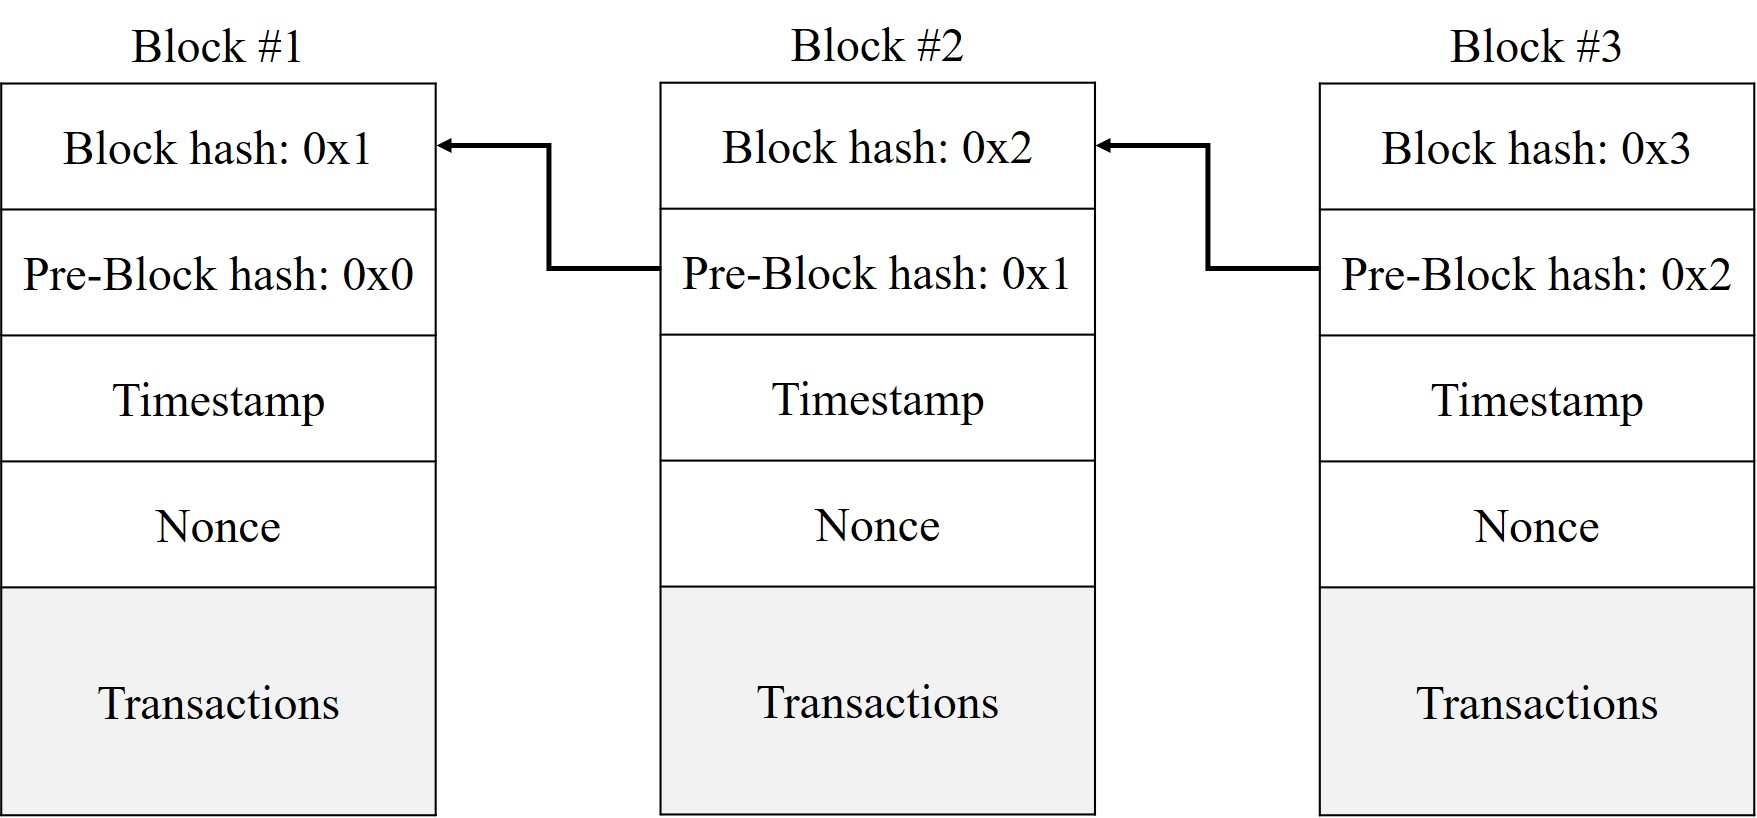
\includegraphics[scale=0.5]{images/1.jpg}
\caption{區塊鏈示意圖}
\label{i:byz-latency}
\end{figure}


因應不同用戶需求及應用場景,區塊鏈系統架構及規模也不盡相同,當前主流應用大致可分為公有鏈以及私有鏈。公有鏈的應用如比特幣或以太坊\cite{Ethereum}等,其特性為任何人都能參與該區塊鏈,加入公有鏈不需要任何人授權,可以隨時自由加入或退出。不同於公有鏈,私有鏈大多是指多個機構共同參與管理的區塊鏈,每個機構執行一或多個節點,參與私有鏈的節點需有嚴格規範。私有鏈的應用如Facebook Libra、R3區塊鏈聯盟等。私有鏈中的資料只允許系統內不同的機構進行讀寫和傳送交易,並且共同記錄及備份資料。由於參與私有鏈的節點是有限制和可控制的,因此私有鏈往往可以有較快的交易速度、更好的隱私保護、且不容易被惡意攻擊,本論文將聚焦於私有鏈上。
因為區塊鏈是一個分散式架構,節點間平權管理,所以需要透過運行相同的「共識協議」來維護相同的區塊順序。這類的共識協議則稱為共識演算法。公有鏈需要有極強的隨機性,大多採工作量證明Proof-of-Work({\em POW})來達成共識。POW透過競賽解題,第一個解出題目的節點將獲得廣播區塊的權力,共識過程中大部分的運算效能都會花在這個解題步驟(俗稱挖礦),因此區塊產出時間會被拉長,導致共識效率低落。然而私有鏈因為節點需經授權才可加入,這類演算法大多透過投票來選擇區塊的廣播者,透過輪流廣播來維持區塊鏈內的平權治理。

私有鏈上通常運行BFT共識演算法,BFT是拜占庭容錯(Byzantine Fault-Tolerant)的縮寫。拜占庭容錯的區塊鏈,能夠在即使系統中部分節點當機或存在惡意節點情況下,保證網絡依舊具備安全性({\em safety})與活性({\em liveness})等性質。Safety能夠保證區塊鏈上每個參與區塊鏈系統的節點都必須擁有相同且排序一致的帳本內容。Liveness則讓區塊鏈是一個永續的系統,能夠容忍錯誤發生,避免因單一節點故障而導致系統停擺。目前已經有許多BFT共識演算法但傳統的BFT演算法通常需要多個回合才能達成共識,每一個回合會有一個節點擔任提議者(Proposer)。一般來說,一個回合需要執行三個步驟。第一個步驟的目的在於讓提議者廣播其提議。若該提議者廣播多份提議,則區塊鏈可能發生分叉(Fork),進而導致內容衝突,這讓攻擊者可能重複花費同一筆金額(Double spending)。第二個步驟的目的即為讓所有節點檢查該提議者是否只有廣播一份提議。若提議者只有廣播一份提議,在第三個步驟中,節點便可以開始投票(將收到的提議廣播給其他節點),若一個節點蒐集到足夠多的同意票,該節點便可以確認該提議為最終共識結果。第三個步驟的目的是為了克服訊息傳輸延遲。知名的BFT演算法PBFT\cite{castro1999practical}便是根據上述三個步驟設計

過去也有少部分的BFT演算法在一個回合中只需要兩個步驟,例子包含FaB\cite{abraham2018revisiting}、Zyzzyva\cite{kotla2007zyzzyva}、SBFT\cite{martin2006fast}、Hydrachain\cite{Hydrachain}。然而,FaB與Zyzzyva已被指出無法保證活性,換句話說,共識演算法可能永遠無法達成共識。另一方面,Hydrachain也被指出無法保證安全性,也就是說,不同的正常節點可能會有不同的共識節果,這在區塊鏈上及代表分岔。雖然SBFT能夠保證安全性與活性,但是SBFT在節點發生故障或是網路延遲過大的情況下,會改用類似PBFT的三步驟設計。因此,在系統狀況良好時,SBFT每回合只需要執行兩個步驟。但是在系統狀況不良時,SBFT每回合仍需要執行三個步驟。
本論文探討的議題為一個新的兩回合拜占庭共識演算法。更明確的說我們希望在不犧牲安全性及活性情況下,設計一個每回合只需要兩個步驟的BFT演算法。重要的是,該BFT演算法即使在系統狀況不佳時,每個回合仍只需要兩個步驟。以下是本篇論本的研究目標: 

\begin{itemize}%项目符号开始
\item 設計一個兩回合的共識演算法FaS-BFT,將該演算法實作於以太坊上並保留以太坊上其他功能。
\item 自動化生成以太坊節點將節點部署模組化,讓系統根據使用者的需求快速搭建該私有鏈。
\item 整合多樣化雲端部署套件快速在雲端伺服器上建立多台環境一致的機器作為私有鏈共識節點。
\item 針對不同實驗環境進行效能測試,進行共識效率比較。 
\end{itemize}





